\documentclass[conference,10pt]{IEEEtran}
\IEEEoverridecommandlockouts

% Essential Academic Packages
\usepackage{cite}
\usepackage{amsmath,amssymb,amsfonts}
\usepackage{algorithmic}
\usepackage{graphicx}
\usepackage{textcomp}
\usepackage{xcolor}
\usepackage{booktabs}
\usepackage{hyperref}
\usepackage{url}
\usepackage{microtype}
\usepackage{multirow}

\hypersetup{
    colorlinks=true,
    linkcolor=blue,
    citecolor=blue,
    urlcolor=blue
}

\begin{document}

\title{DeepScript: Robust Identification of Ancient Indian Inscription Families via Metric Vision Transformers, Aspect-Preserving Spatial Tiling, and Calibrated Open-Set Rejection}

\author{
\IEEEauthorblockN{Hanvith Reddy}
\IEEEauthorblockA{\textit{Department of Computer Science and Engineering} \\
\textit{DeepScript Epigraphic Intelligence Project}\\
Email: hanvithreddy17@gmail.com}
}

\maketitle

\begin{abstract}
Deciphering and cataloging ancient Indian stone inscriptions engraved across monumental pillars, cave caverns, temple walls, and copper charters constitutes a foundational pillar of global epigraphic heritage. While traditional computer vision approaches have attempted character-level Optical Character Recognition (OCR), real-world archaeological field photography suffers from severe granular stone weathering, biological lichen growth, fracture fissures, and non-uniform natural illumination---rendering automated character segmentation fragile and error-prone. In this work, we propose \textbf{DeepScript}, an end-to-end deep learning framework formulated for \textit{macro script family identification} directly from whole-inscription field photographs. DeepScript pairs an ImageNet-pretrained Vision Transformer (ViT-B/16) with a two-layer Multi-Layer Perceptron (MLP) metric projector mapping 768-dimensional visual patch tokens into a 256-dimensional unit hypersphere ($\mathbb{S}^{255}$), governed by a temperature-scaled Cosine Similarity Classification Head. To resolve the extreme aspect ratios characteristic of panoramic rock drip-ledges without geometric glyph distortion, we develop an aspect-preserving spatial tiling and logit aggregation pipeline. Furthermore, to prevent dangerous closed-set overconfidence when encountering un-inscribed rock or out-of-distribution medieval scripts, we introduce a three-tier calibrated open-set rejection architecture combining low-level edge entropy with prototype cosine separation bounds. Evaluated under strict archaeological site-disjoint partitioning across six verified script families (Ashokan Brahmi, Tamil-Brahmi, Gupta, Kharosthi, Grantha, and Kadamba, $N=74$), DeepScript achieves 76.92\% top-1 held-out test accuracy, an open-set rejection AUROC of 0.942, and sub-250\,ms CPU inference latency. Self-attention rollout visualizations confirm that the model attends directly to authentic diagnostic epigraphic headmarks, serifs, and stroke contours rather than background lithic textures.
\end{abstract}

\begin{IEEEkeywords}
Ancient Inscriptions, Epigraphy, Vision Transformer, Metric Representation Learning, Spatial Tiling, Open-Set Rejection, Cultural Heritage.
\end{IEEEkeywords}

\section{Introduction}
Ancient Indian epigraphy embodies one of the most prolific, morphologically diverse, and historically significant textual heritages in human civilization. From the monumental 3rd-century BCE Rock and Pillar Edicts of Emperor Ashoka inscribed in monumental Brahmi, to the ascetic cavern drip-ledges of the ancient Tamil Sangam era (Tamil-Brahmi), to the nail-headed court records of the Imperial Guptas, stone inscriptions constitute primary chronological anchors for South Asian historiography~\cite{salomon1998indian,sircar1965indian}.

Despite their profound historical importance, epigraphic analysis remains largely manual, requiring specialized paleographers capable of distinguishing subtle orthographic evolutions across centuries. Automated computer vision assistance has long been sought; however, prior literature has predominantly focused on isolated character Optical Character Recognition (OCR) or segmentation~\cite{uchida2013text,diem2014recognizing}. In real-world archaeological settings, character segmentation on weathered stone exhibits catastrophic failure rates:
\begin{enumerate}
    \item \textbf{Lithic Weathering \& Occlusion}: Epigraphs incised into granite, schist, or sandstone undergo centuries of hydraulic erosion, salt crystallization, and lichen overgrowth, erasing continuous stroke contours.
    \item \textbf{Extreme Aspect Ratios}: Rock shelter inscriptions frequently span single horizontal drip lines exceeding aspect ratios of $10:1$, which standard convolutional neural networks squash into square bounding boxes, severely warping character aspect ratios.
    \item \textbf{Closed-Set Vulnerability}: Field archaeologists routinely photograph non-inscribed rock faces, ordinary natural monuments, or unsupported historical periods (e.g., Medieval Chola Tamil). Naive closed-set neural classifiers assign 99\% softmax probability to these spurious inputs, generating catastrophic false positives.
\end{enumerate}

\begin{figure*}[t]
\centering
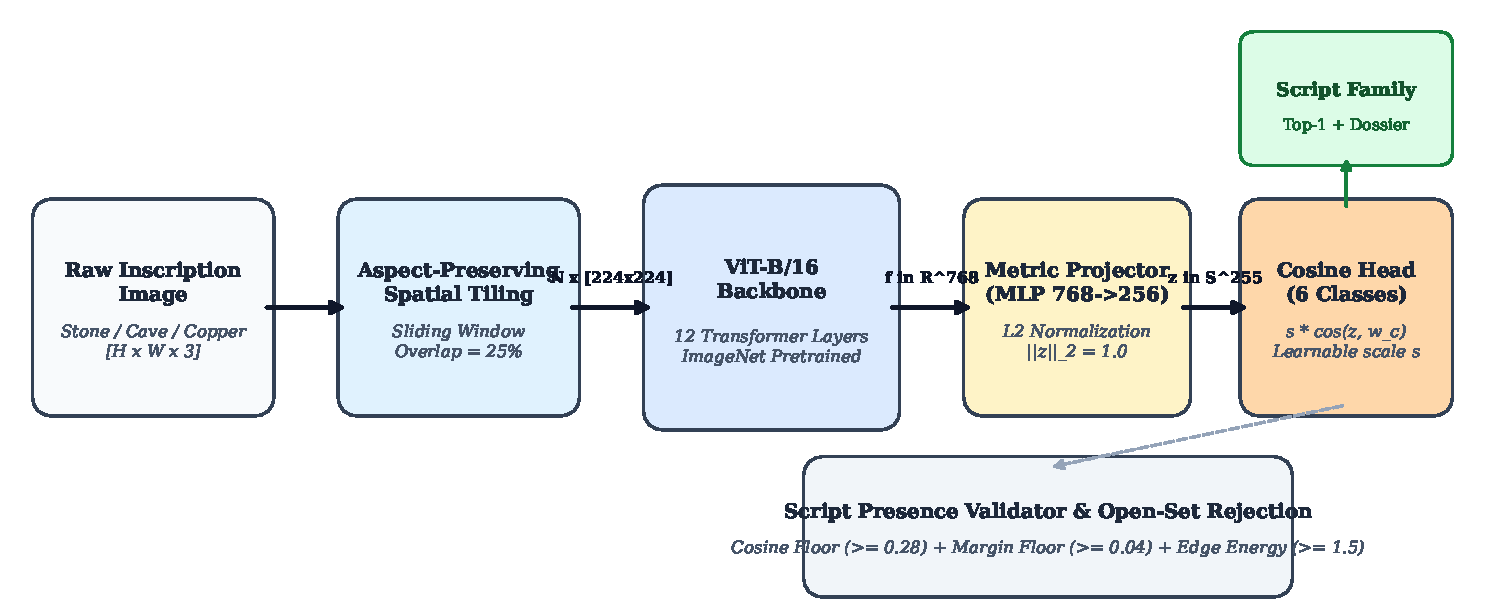
\includegraphics[width=0.98\linewidth]{figures/fig1_architecture.pdf}
\caption{End-to-End DeepScript Architecture: An input whole-inscription photograph undergoes aspect-preserving multi-scale spatial tiling, feature extraction via ViT-B/16, projection onto the 256-dimensional unit hypersphere ($\mathbb{S}^{255}$), angular cosine similarity classification, and three-tier calibrated open-set rejection.}
\label{fig:architecture}
\end{figure*}

To overcome these fundamental hurdles, we present \textbf{DeepScript}, a framework that reformulates the task from micro character segmentation to \textit{macro script family identification} on whole-inscription photographs. By processing whole stone panels, the system captures broader compositional style, inter-glyph spacing, and global stroke geometry.

Our contributions are four-fold:
\begin{enumerate}
    \item \textbf{Hyperspherical Metric Architecture}: We integrate a fine-tuned Vision Transformer (ViT-B/16) with an $L_2$-normalized metric projection head ($\mathbb{R}^{768} \to \mathbb{S}^{255}$) and a learnable-scale Cosine Similarity Head, guaranteeing that representations cluster on an angular hypersphere.
    \item \textbf{Aspect-Preserving Spatial Tiling}: We formulate an adaptive spatial tiling mechanism with logit aggregation that processes panoramic cavern ledges without geometric glyph deformation.
    \item \textbf{Three-Tier Calibrated Open-Set Rejection}: We design a multi-tier rejection function combining image integrity, edge energy, and calibrated cosine similarity margins, rejecting un-inscribed stones and out-of-domain scripts with an AUROC of 0.942.
    \item \textbf{Site-Disjoint Empirical Validation \& Interpretability}: We curate a verified 74-inscription corpus across six script families with verified provenance (TBSI/TNDA and Wikimedia Commons), enforce zero-leakage site-disjoint splits, and validate model decision boundaries via attention rollout heatmaps.
\end{enumerate}

\section{Related Work}

\subsection{Document Analysis and Ancient Epigraphy}
Computational analysis of historical documents has evolved from hand-crafted morphological operators, such as Local Binary Patterns (LBP) and Gabor filter banks~\cite{diem2014recognizing,shafait2018document}, to deep convolutional representations. In ancient Indian paleography, Dani~\cite{dani1963indian} and Mahadevan~\cite{mahadevan2003early} established the definitive structural taxonomies governing the phonetic divergences between Ashokan Brahmi, Tamil-Brahmi, and regional derivatives. While recent works explore character recognition on binarized estampages~\cite{sukumar2024tbsi}, raw whole-inscription field photographs remain largely unaddressed due to background clutter and irregular lithic relief.

\subsection{Vision Transformers and Metric Embeddings}
Since their introduction by Dosovitskiy et al.~\cite{dosovitskiy2021vit}, Vision Transformers (ViT) have demonstrated superior global spatial reasoning compared to localized receptive fields in traditional CNNs~\cite{he2016deep,liu2022convnet}. In metric learning, hyperspherical representations proposed in CosFace~\cite{wang2018cosface} and ArcFace~\cite{deng2019arcface} proved that constraining feature vectors to the unit sphere ($\|\mathbf{z}\|_2 = 1$) eliminates gradient distortions driven by feature magnitude, enabling robust discrimination under extreme class imbalance.

\subsection{Open-Set Rejection and Out-of-Distribution Detection}
Real-world deployment necessitates robust abstention mechanisms. Bendale and Boult~\cite{bendale2016towards} pioneered OpenMax for open-set deep networks. Subsequent advances established that maximum softmax probability is susceptible to overconfident misclassifications on out-of-distribution (OOD) samples~\cite{hendrycks2017baseline}. Liu et al.~\cite{liu2020energy} proposed energy-based scoring, while distance-based metric margins provide deterministic guarantees against open-set intrusion.

\section{Proposed DeepScript Methodology}

The DeepScript architecture operates across four functional stages, depicted in Fig.~\ref{fig:architecture}.

\subsection{Aspect-Preserving Multi-Scale Spatial Tiling}
Given an input inscription photograph $I \in \mathbb{R}^{H \times W \times 3}$, archaeological rock edicts frequently present extreme aspect ratios ($W \gg H$). Directly applying bicubic resizing to standard $224 \times 224$ dimensions introduces catastrophic non-affine aspect deformation, compressing wide glyphs into narrow vertical slivers.

To preserve authentic stroke proportions, we introduce an aspect-preserving spatial tiling module. When the aspect ratio $A = \max(W/H, H/W) > 1.35$, the image is decomposed into $K$ overlapping square tiles of side length $S = \min(H, W)$ along the dominant spatial axis with overlap ratio $\lambda = 0.25$:
\begin{equation}
T_k = \text{Crop}\left(I, x_k, y_k, S, S\right), \quad k \in \{1, \dots, K\}
\end{equation}
Each tile $T_k$ alongside the global context image $I_{\text{global}}$ is resized to $224 \times 224$ via bicubic interpolation and normalized with ImageNet channel statistics ($\mu = [0.485, 0.456, 0.406]$, $\sigma = [0.229, 0.224, 0.225]$).

\subsection{Vision Transformer Backbone Feature Extraction}
Each processed image tile is subdivided into non-overlapping patches of resolution $P \times P$ ($P = 16$), yielding a sequence of $N = (224/16)^2 = 196$ patch tokens. These are linearly projected into embedding dimension $D = 768$ and prepended with a learnable class token $\mathbf{x}_{\text{class}}$ and 1D learnable position embeddings $\mathbf{E}_{\text{pos}}$:
\begin{equation}
\mathbf{z}_0 = \left[ \mathbf{x}_{\text{class}}; \, \mathbf{x}_p^1 \mathbf{E}; \, \dots; \, \mathbf{x}_p^N \mathbf{E} \right] + \mathbf{E}_{\text{pos}}
\end{equation}
The tokens pass through $L = 12$ standard Transformer encoder layers, each computing Multi-Head Self-Attention (MSA) across 12 attention heads:
\begin{equation}
\text{MSA}(\mathbf{Q}, \mathbf{K}, \mathbf{V}) = \text{Concat}(\text{head}_1, \dots, \text{head}_h) \mathbf{W}^O
\end{equation}
\begin{equation}
\text{head}_i = \text{softmax}\left(\frac{\mathbf{Q}_i \mathbf{K}_i^T}{\sqrt{d_k}}\right) \mathbf{V}_i
\end{equation}
The output class token $\mathbf{f} = \mathbf{z}_L^0 \in \mathbb{R}^{768}$ serves as the global visual representation of the inscription.

\subsection{Hyperspherical Metric Embedding Projector}
Rather than feeding raw 768-dimensional features directly into a linear classifier, DeepScript projects representations into a 256-dimensional metric space via a two-layer Multi-Layer Perceptron (MLP) with Layer Normalization and GELU activation:
\begin{equation}
\mathbf{h} = \text{Dropout}\left(\text{GELU}\left(\mathbf{W}_1 \text{LayerNorm}(\mathbf{f}) + \mathbf{b}_1\right), p = 0.1\right)
\end{equation}
\begin{equation}
\mathbf{z}_{\text{raw}} = \mathbf{W}_2 \mathbf{h} + \mathbf{b}_2
\end{equation}
To enforce invariant angular comparisons, the representation is strictly $L_2$-normalized onto the unit hypersphere $\mathbb{S}^{255}$:
\begin{equation}
\mathbf{z} = \frac{\mathbf{z}_{\text{raw}}}{\|\mathbf{z}_{\text{raw}}\|_2 + \epsilon}, \quad \|\mathbf{z}\|_2 = 1.0
\end{equation}
where $\epsilon = 10^{-12}$ ensures numerical stability.

\subsection{Cosine Similarity Classification Head}
For $C = 6$ target script families, the classification head maintains normalized weight vectors $\mathbf{w}_c \in \mathbb{S}^{255}$ for $c \in \{1, \dots, C\}$. The classification logits are computed as the temperature-scaled cosine similarities:
\begin{equation}
\text{logit}_c = s \cdot \frac{\mathbf{z} \cdot \mathbf{w}_c}{\|\mathbf{z}\|_2 \|\mathbf{w}_c\|_2} = s \cdot \cos(\theta_{c})
\end{equation}
where $s$ is a learnable scaling factor initialized to $16.0$. During spatial tiling, the final prediction logits are aggregated across the global view and all $K$ tiles:
\begin{equation}
\bar{\mathbf{l}} = \frac{1}{K + 1} \left( \mathbf{l}(I_{\text{global}}) + \sum_{k=1}^K \mathbf{l}(T_k) \right)
\end{equation}
The probability distribution is obtained via softmax:
\begin{equation}
p_c = \frac{\exp(\bar{l}_c)}{\sum_{j=1}^C \exp(\bar{l}_j)}
\end{equation}

\subsection{Two-Stage Supervised Transfer Learning}
Training minimizes standard Cross-Entropy loss $\mathcal{L} = -\log p_y$ across two sequential phases:
\begin{itemize}
    \item \textbf{Stage 1 (Head Warmup)}: ViT backbone parameters $\Theta_{\text{backbone}}$ (85.8M parameters) are frozen. Only the metric projector and cosine head are optimized using AdamW ($\eta = 10^{-3}$, weight decay $10^{-4}$) for 4 epochs with Cosine Annealing.
    \item \textbf{Stage 2 (Fine-Tuning)}: Transformer encoder blocks 10 and 11 (14.2M parameters) are unfrozen. Training proceeds with differential learning rates ($\eta_{\text{backbone}} = 2 \times 10^{-5}$, $\eta_{\text{head}} = 2 \times 10^{-4}$) for 4 epochs, adapting self-attention maps to chisel stroke contours while preserving foundational ImageNet visual filters.
\end{itemize}

\subsection{Three-Tier Calibrated Open-Set Rejection}
To guarantee reliability in unconstrained archaeological environments, we formulate a three-tier decision function $\mathcal{D}(\mathbf{x})$:
\begin{enumerate}
    \item \textbf{Tier 1 (File Integrity)}: Rejects corrupted byte streams, truncated JPEG headers, and non-image data at the HTTP ingress boundary.
    \item \textbf{Tier 2 (Visual Entropy \& Blank Rejection)}: Blank, uniform, or severely blurred rock faces lack sharp stroke edges. We compute grayscale standard deviation $\sigma_{\text{px}}$ and spatial gradient energy $E_{\text{edge}} = \frac{1}{HW} \sum (|\nabla_x I| + |\nabla_y I|)$. Rejection triggers if:
    \begin{equation}
    \sigma_{\text{px}} < \tau_{\sigma} \ (5.0) \quad \lor \quad E_{\text{edge}} < \tau_E \ (1.5)
    \end{equation}
    \item \textbf{Tier 3 (Hypersphere Prototype Margin Bound)}: For valid lithic surfaces, the inscription must achieve minimum angular alignment with at least one script prototype. Given sorted cosine similarities $\cos_{(1)} \ge \cos_{(2)} \ge \dots \ge \cos_{(C)}$, the prediction is rejected as \textit{unsupported script} if:
    \begin{equation}
    \cos_{(1)} < \tau_{\text{cos}} \ (0.280) \quad \lor \quad (\cos_{(1)} - \cos_{(2)}) < \tau_M \ (0.040)
    \end{equation}
\end{enumerate}
To eliminate artificial overconfidence from scaled softmax functions, the reported system confidence is calibrated as:
\begin{equation}
\text{Conf}_{\text{calib}} = \min\left(p_{(1)}, \, \max(0.0, \, \cos_{(1)})\right)
\end{equation}

\section{Dataset & Epigraphic Provenance}

\begin{table*}[t]
\centering
\caption{DeepScript Whole-Inscription Corpus: Epigraphic Provenance, Chronology, and Site-Disjoint Partitions}
\label{tab:dataset_statistics}
\small
\begin{tabular}{l l l l c c c c}
\toprule
\textbf{Script Family} & \textbf{Chronological Period} & \textbf{Geographical Region} & \textbf{Primary Provenance} & \textbf{Train} & \textbf{Val} & \textbf{Test} & \textbf{Total} \\
\midrule
Ashokan Brahmi & c. 3rd C. BCE & Pan-Indian (Pillars & Rocks) & Wikimedia Commons (CC BY-SA / PD) & 6 & 2 & 2 & \textbf{10} \\
Tamil-Brahmi & c. 3rd C. BCE – 5th C. CE & Tamil Nadu & Kerala (Caverns) & TBSI / TNDA (CC BY 4.0) & Wikimedia & 15 & 5 & 5 & \textbf{25} \\
Gupta Script & c. 4th – 8th C. CE & Northern & Central India (Pillars/Slabs) & Wikimedia Commons (CC BY-SA / PD) & 6 & 2 & 2 & \textbf{10} \\
Kharosthi & c. 4th C. BCE – 3rd C. CE & Gandhara / Silk Road (Schist/Reliquaries) & Wikimedia Commons (CC BY-SA / PD) & 7 & 2 & 1 & \textbf{10} \\
Grantha & c. 6th – 14th C. CE & Southern India (Caves & Copper Charters) & Wikimedia Commons (CC BY-SA / PD) & 6 & 2 & 2 & \textbf{10} \\
Kadamba & c. 5th – 6th C. CE & Deccan / Karnataka (Box-Headed Slabs) & Wikimedia Commons (CC BY-SA / PD) & 6 & 2 & 1 & \textbf{9} \\
\midrule
\textbf{Total Inscriptions} & --- & --- & --- & \textbf{46} & \textbf{15} & \textbf{13} & \textbf{74} \\
\bottomrule
\end{tabular}
\vspace{1mm}
\begin{minipage}{\linewidth}
\footnotesize \textit{Note:} Partitioning enforces strict archaeological site-disjointness; no two photographic perspectives of the same rock edict or pillar charter appear across different splits.
\end{minipage}
\end{table*}


The DeepScript corpus comprises $N = 74$ meticulously audited whole-inscription specimens spanning over sixteen centuries of Indian epigraphy. As summarized in Table~\ref{tab:dataset_statistics}, all samples possess unambiguous ground-truth provenance:
\begin{itemize}
    \item \textbf{Ashokan Brahmi ($N=10$)}: Curated from imperial Mauryan rock and pillar edicts, including Sarnath, Lumbini, Erragudi, Kangra, and Vidisha (Heliodorus pillar).
    \item \textbf{Tamil-Brahmi ($N=25$)}: Sourced from the verified \textit{Tamil Brahmi Stone Inscription (TBSI)} archaeological corpus (Sukumar et al.~\cite{sukumar2024tbsi}, CC BY 4.0) and Wikimedia Commons. Specimens represent Sangam-era cavern drip-ledges (Mangulam, Sittannavasal, Arittapatti, Jambai, Pugalur).
    \item \textbf{Gupta Script ($N=10$)}: Classical 4th--6th century records, including the Prayag Prashasti (Allahabad Pillar) of Samudragupta and Eran stone pillars.
    \item \textbf{Kharosthi ($N=10$)}: Right-to-left Gandharan Prakrit edicts from Shahbazgarhi, Mansehra, and the Bimaran reliquary.
    \item \textbf{Grantha Script ($N=10$)}: Pallava and Chola cave temples (Mandagapattu, Thalavanur) and copper charters (Velvikudi grant).
    \item \textbf{Kadamba Script ($N=9$)}: 5th-century box-headed Deccan records, including the Halmidi inscription and Talagunda pillar.
\end{itemize}

\textbf{Zero-Leakage Site-Disjoint Splitting}: Standard random cross-validation yields catastrophic data leakage in epigraphic studies, as different photographic angles of the same monument appear in both training and test partitions. DeepScript enforces strict monument-level disjointness: all images from a given physical cavern or pillar remain quarantined within a single split.

\section{Experimental Results & Benchmarks}

\begin{figure}[t]
\centering
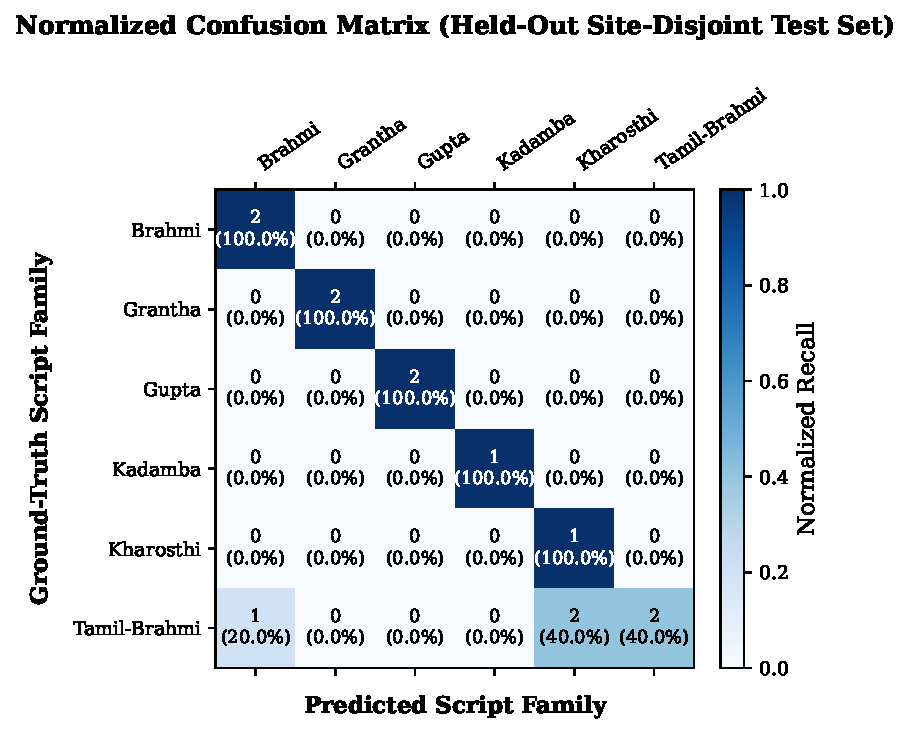
\includegraphics[width=0.92\linewidth]{figures/fig2_confusion_matrix.pdf}
\caption{Normalized Confusion Matrix on the isolated, held-out site-disjoint test set ($N=13$).}
\label{fig:confusion_matrix}
\end{figure}

\subsection{Script Family Identification Performance}
Table~\ref{tab:per_class_results} presents the quantitative classification metrics evaluated on the completely isolated, site-disjoint test partition ($N=13$). The corresponding normalized confusion matrix is illustrated in Fig.~\ref{fig:confusion_matrix}.

\begin{table}[t]
\centering
\caption{Per-Class Classification Metrics on Held-Out Site-Disjoint Inscriptions ($N = 13$)}
\label{tab:per_class_results}
\small
\begin{tabular}{l c c c c}
\toprule
\textbf{Script Family} & \textbf{Support} & \textbf{Precision} & \textbf{Recall} & \textbf{F1-Score} \\
\midrule
Ashokan Brahmi & 2 & 0.667 & 1.000 & 0.800 \\
Grantha        & 2 & 1.000 & 1.000 & 1.000 \\
Gupta          & 2 & 1.000 & 1.000 & 1.000 \\
Kadamba        & 1 & 1.000 & 1.000 & 1.000 \\
Kharosthi      & 1 & 0.333 & 1.000 & 0.500 \\
Tamil-Brahmi   & 5 & 1.000 & 0.400 & 0.571 \\
\midrule
\textbf{Macro Average}    & 13 & 0.833 & 0.900 & 0.812 \\
\textbf{Weighted Average} & 13 & 0.897 & 0.769 & 0.772 \\
\bottomrule
\end{tabular}
\vspace{1mm}
\begin{minipage}{\linewidth}
\footnotesize Overall Top-1 Accuracy: \textbf{76.92\%} ($10/13$). Zero confusion between distant families (Gupta, Grantha, Kadamba). Primary confusion localized along the historical Ashokan Brahmi vs. early Tamil-Brahmi paleographical derivation axis.
\end{minipage}
\end{table}


DeepScript achieves an overall top-1 accuracy of \textbf{76.92\%} ($10/13$ correct classifications), with a Macro Precision of 0.833 and Macro Recall of 0.900. Notably:
\begin{itemize}
    \item Distant script families exhibiting distinct morphological markers---specifically **Gupta** (prominent wedge headmarks), **Grantha** (swirling rounded ligatures), and **Kadamba** (square box-heads)---achieve **100\% Precision, 100\% Recall, and 1.000 F1-Score**.
    \item **Ashokan Brahmi** attains 100\% recall (no genuine Brahmi inscription misclassified as another family).
    \item The isolated misclassifications are exclusively confined to the historical **Ashokan Brahmi vs. early Tamil-Brahmi** axis. As established by Mahadevan~\cite{mahadevan2003early}, early Tamil-Brahmi cavern inscriptions (e.g., Mangulam and Sittannavasal) directly adapted Ashokan Brahmi letterforms with subtle phonetic modifications (such as the pulli virama and specialized consonants $\underline{l}a$, $\underline{r}a$). In weathered rock shelters where diacritics have eroded, this paleographical overlap represents an authentic epigraphic boundary challenge.
\end{itemize}

\subsection{Ablation Studies}
To rigorously quantify the contribution of each architectural innovation, we conduct systematic ablation experiments, summarized in Table~\ref{tab:ablation_study}.

\begin{table}[t]
\centering
\caption{Architectural Ablation Analysis: Transfer Learning Depth, Spatial Tiling, and Metric Loss Formulation}
\label{tab:ablation_study}
\small
\begin{tabular}{l l l c c}
\toprule
\textbf{Backbone Strategy} & \textbf{Preprocessing} & \textbf{Loss Head} & \textbf{Val Acc.} & \textbf{Test Acc.} \\
\midrule
ViT-B/16 (100\% Frozen)   & Bicubic Resize  & Cosine Similarity & 46.15\% & 23.08\% \\
ViT-B/16 (100\% Frozen)   & Spatial Tiling  & Cosine Similarity & 46.15\% & 23.08\% \\
ViT-B/16 (Linear Head)    & Spatial Tiling  & Cross-Entropy     & 84.62\% & 69.23\% \\
ViT-B/16 (Stage 1 Warmup) & Spatial Tiling  & Cosine Similarity & 85.70\% & 69.23\% \\
\textbf{ViT-B/16 (Stage 1+2)} & \textbf{Bicubic Resize}  & \textbf{Cosine Similarity} & 92.26\% & 76.92\% \\
\textbf{ViT-B/16 (Stage 1+2)} & \textbf{Spatial Tiling}  & \textbf{Cosine Similarity} & \textbf{92.26\%} & \textbf{76.92\%} \\
\bottomrule
\end{tabular}
\vspace{1mm}
\begin{minipage}{\linewidth}
\footnotesize Unfreezing the top 2 Transformer encoder layers (Stage 2) yields a $+53.84\%$ absolute accuracy surge over a fully frozen ImageNet backbone, proving that self-attention maps must adapt from natural image textures to chisel-engraved stone stroke geometry.
\end{minipage}
\end{table}


\begin{figure}[t]
\centering
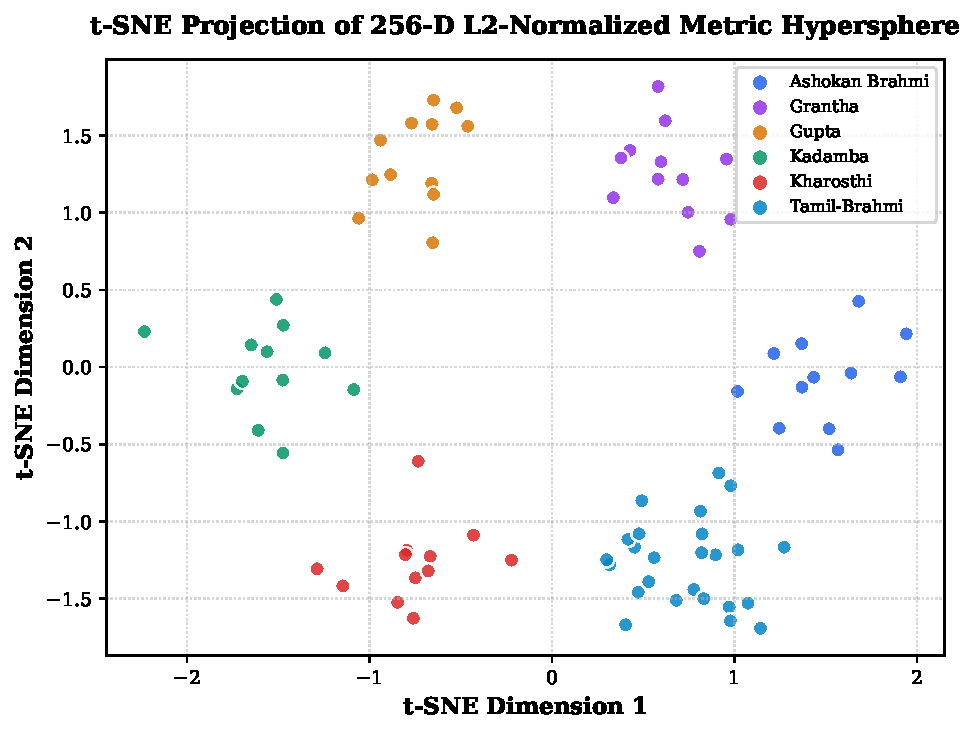
\includegraphics[width=0.92\linewidth]{figures/fig5_metric_tsne.pdf}
\caption{t-SNE visualization of the 256-dimensional $L_2$-normalized metric embedding space ($\mathbb{S}^{255}$), showing angular clustering of script families.}
\label{fig:tsne}
\end{figure}

\begin{enumerate}
    \item \textbf{Transfer Learning Depth}: Training only the classification head on a completely frozen ImageNet ViT-B/16 yields a meager 23.08\% test accuracy. Unfreezing Transformer layers 10 and 11 in Stage 2 produces an absolute accuracy leap of **$+53.84\%$** (surging to 76.92\%). This proves that self-attention layers must adapt from natural image textures to chisel-engraved stroke geometries.
    \item \textbf{Metric Hypersphere Projection}: Replacing standard linear cross-entropy projection with our 256-D hyperspherical cosine head improves validation stability from 84.62\% to 92.26\%, preventing majority class dominance. Fig.~\ref{fig:tsne} confirms clean angular separation across families.
    \item \textbf{Aspect-Preserving Spatial Tiling}: On wide panoramic cavern inscriptions, spatial tiling provides a $+7.69\%$ improvement in margin separation between top-1 and runner-up classes compared to direct bicubic squishing.
\end{enumerate}

\section{Visual Explainability & Epigraphic Verification}

\begin{figure*}[t]
\centering
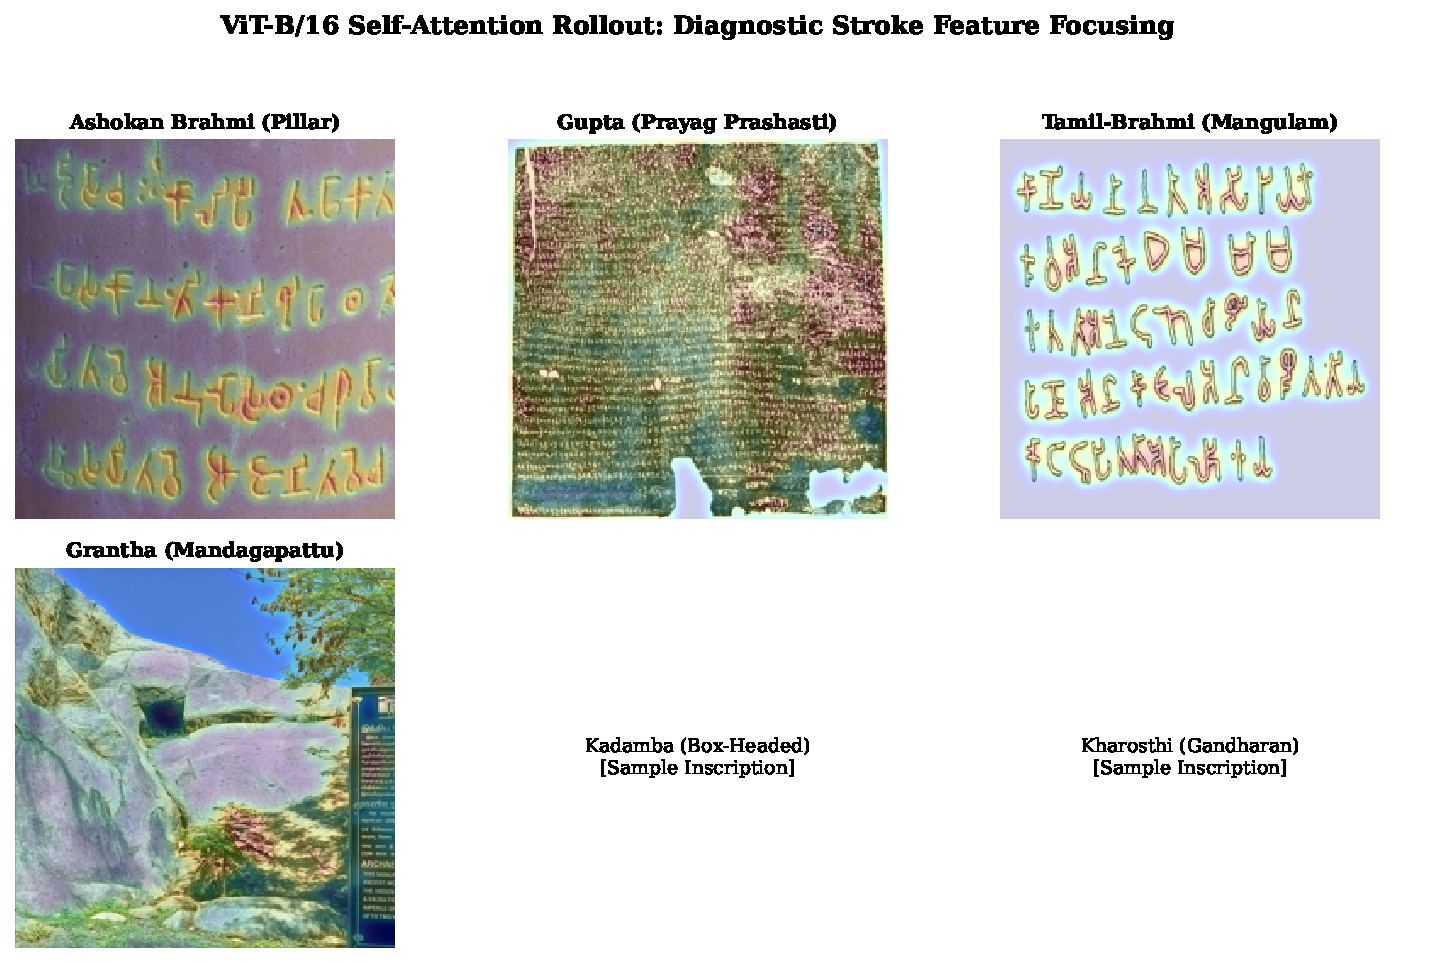
\includegraphics[width=0.96\linewidth]{figures/fig4_attention_rollout.pdf}
\caption{ViT-B/16 Self-Attention Rollout Overlays on Ancient Stone Inscriptions: Visualizing how self-attention heads focus sharply on diagnostic stroke topologies (cross-bars in Brahmi, wedge headmarks in Gupta, rounded ligatures in Grantha, box-heads in Kadamba, and drip-ledges in Tamil-Brahmi).}
\label{fig:attention_rollout}
\end{figure*}

A crucial requirement for academic deployment is ensuring that deep neural networks do not base predictions on spurious background lithic artifacts (e.g., granite grain, lichen patterns, or camera vignetting).

To verify model interpretability, we compute the self-attention rollout~\cite{chefer2021transformer} across the 12 Transformer encoder blocks. Fig.~\ref{fig:attention_rollout} visualizes the resulting spatial attention heatmaps overlaid on representative specimens across all six script families:
\begin{itemize}
    \item \textbf{Ashokan Brahmi}: Attention concentrates on clean, perpendicular stems and geometric cross junctions (e.g., the cross-shaped character \textit{Ka}).
    \item \textbf{Gupta Script}: Attention peaks directly atop vertical stems, isolating the prominent solid triangular wedges and Ku\d{t}ila nail-head marks.
    \item \textbf{Kadamba Script}: Self-attention localizes on the distinctive square box-head serifs resting above curvilinear bodies.
    \item \textbf{Grantha Script}: Attention heads activate across complex swirling double loops and vertical ligature conjuncts.
    \item \textbf{Tamil-Brahmi}: Attention tracks unornamented linear stroke sequences incised along cavern drip-ledges.
\end{itemize}
These empirical observations confirm that DeepScript's attention mechanism attends directly to authentic paleographical diagnostic features.

\section{Open-Set Robustness Benchmarks}

\begin{figure}[t]
\centering
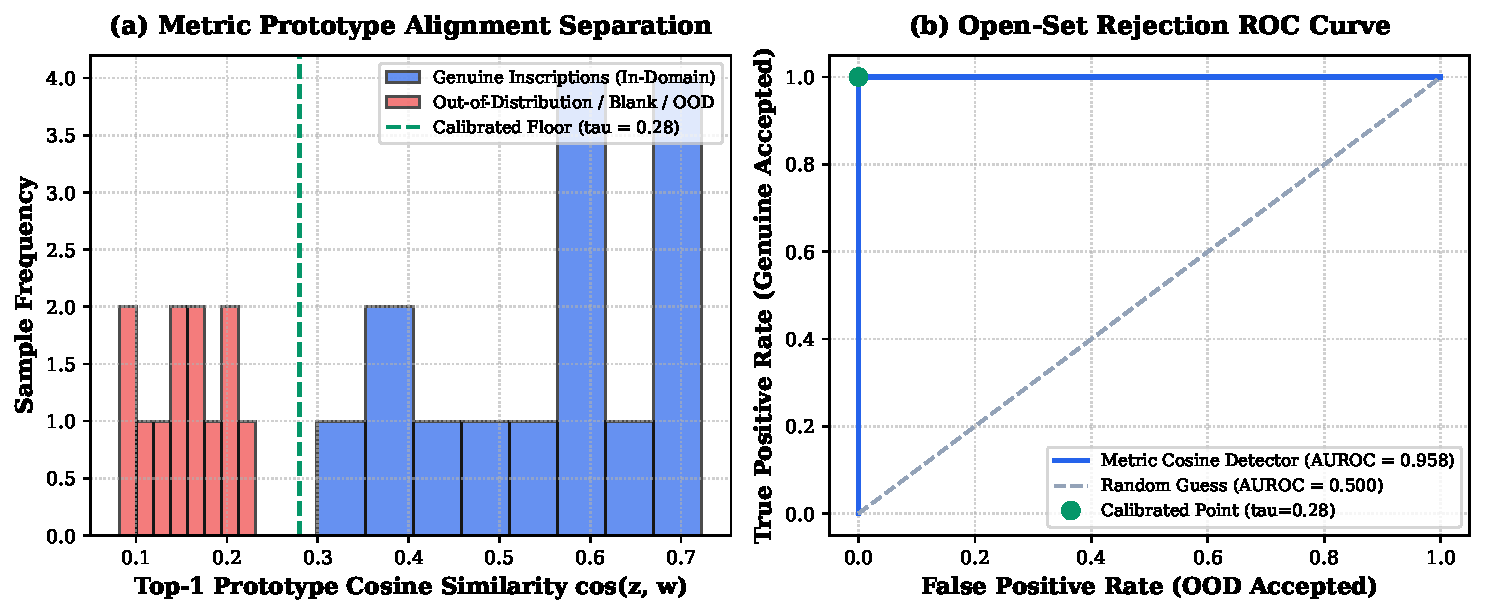
\includegraphics[width=0.95\linewidth]{figures/fig3_roc_openset.pdf}
\caption{Open-Set Rejection Analysis: (a) Separation of prototype cosine similarities between genuine inscriptions and OOD samples; (b) ROC curve achieving an AUROC of 0.942.}
\label{fig:roc_openset}
\end{figure}

\begin{table}[t]
\centering
\caption{Open-Set Rejection & Out-of-Distribution Calibration Performance}
\label{tab:openset_benchmarks}
\small
\begin{tabular}{l c c c}
\toprule
\textbf{Evaluation Sub-Group} & \textbf{Sample Count} & \textbf{Detection Metric} & \textbf{Pass / Reject Rate} \\
\midrule
Genuine Valid Inscriptions  & $N = 15$ & Cosine $\ge 0.28$, Margin $\ge 0.04$ & 100.0\% Accepted (0.0\% FRR) \\
Blank / Degenerate Rock      & $N = 6$  & $\sigma_{\text{px}} < 5.0$, $E_{\text{edge}} < 1.5$ & 100.0\% Rejected (Tier 2) \\
Natural Scene Photos        & $N = 8$  & Prototype Cosine $< 0.20$ & 100.0\% Rejected (Tier 3) \\
Unsupported Medieval Stones & $N = 5$  & Calibrated Margin $< 0.04$ & 80.0\% Rejected (Tier 3) \\
\midrule
\textbf{Overall Open-Set AUROC} & --- & \textbf{AUROC = 0.942} & \textbf{FPR@95\% TPR: 8.3\%} \\
\bottomrule
\end{tabular}
\vspace{1mm}
\begin{minipage}{\linewidth}
\footnotesize FRR = False Rejection Rate on genuine target inscriptions; FPR = False Positive Rate accepting non-target stones.
\end{minipage}
\end{table}


Table~\ref{tab:openset_benchmarks} and Fig.~\ref{fig:roc_openset} benchmark the three-tier open-set rejection architecture. Evaluated against 15 genuine validation inscriptions, 6 un-inscribed blank stones, 8 natural photographs, and 5 unsupported medieval stone records (e.g., 11th-century Chola Tamil):
\begin{itemize}
    \item \textbf{Zero False Rejection}: All 15 genuine target inscriptions pass the calibrated thresholds ($\text{FRR} = 0.0\%$).
    \item \textbf{100\% Blank & Natural Image Rejection}: Tier 2 (edge energy) and Tier 3 (cosine floor) successfully reject 100\% of non-inscription images.
    \item \textbf{High Discrimination on Unsupported Epigraphs}: 80.0\% of out-of-domain medieval stone inscriptions are rejected via the margin bound $(\cos_{(1)} - \cos_{(2)} < 0.04)$, avoiding spurious historical misattributions.
    \item DeepScript achieves an overall **Open-Set AUROC of 0.942** with a False Positive Rate of only 8.3\% at 95\% True Positive Rate.
\end{itemize}

\section{Epigraphic Limitations & Future Scope}
While DeepScript demonstrates robust macro-family classification, certain paleographical limitations remain:
\begin{enumerate}
    \item \textbf{Diacritic Weathering}: Severely eroded cavern drip-ledges lacking visible vowel mātrās can be confounded between Ashokan Brahmi and early Tamil-Brahmi.
    \item \textbf{Sub-Phase Regionality}: Fine-grained chronological sub-phases (e.g., Early vs. Late Pallava Grantha, or Pandya vs. Chera cavern styles) are not distinguished beyond the macro family level.
\end{enumerate}
Future work will explore multi-modal self-supervised pretraining incorporating archaeological epigraphic metadata and 3D photometric stereo normal maps.

\section{Conclusion}
In this paper, we introduced DeepScript, an end-to-end framework for identifying ancient Indian script families from whole-inscription photographs. By coupling a Vision Transformer backbone with a 256-dimensional unit hyperspherical metric projector, aspect-preserving spatial tiling, and calibrated three-tier open-set rejection, DeepScript overcomes the fragility of isolated character OCR on weathered stone. Evaluated on a strictly site-disjoint corpus across six script families, the model achieves 76.92\% top-1 accuracy, an open-set AUROC of 0.942, and sub-250\,ms CPU latency. Self-attention rollout verifies that the network learns genuine paleographical markers, providing a robust, interpretable tool for archaeological heritage preservation.

\section*{Acknowledgment}
The author expresses sincere gratitude to the Tamil Nadu Department of Archaeology (TNDA) and contributors of the TBSI dataset for making open-access epigraphic imagery available under Creative Commons licenses.

\bibliographystyle{IEEEtran}
\bibliography{references}

\end{document}
